% Gabarit pandoc des corrigés publiés (brut et guidé). Contenu sans marque ni nom de site.
% Compilation : lualatex (latexmk -lualatex).
% Le Markdown reste la source unique : ne pas éditer ce fichier .tex à la main.
\documentclass[11pt,a4paper]{article}

% --- Moteur, polices (Latin Modern) et langue ---------------------------------
\usepackage{iftex}
\ifLuaTeX\else\errmessage{Ce document se compile avec lualatex}\fi
\usepackage{amsmath,amssymb,mathtools}
\usepackage{fontspec}
% mathrm=sym : \mathrm prend ses glyphes dans la police mathématique (ℓ, μ, Ω), comme KaTeX.
\usepackage[math-style=TeX,bold-style=TeX,mathrm=sym]{unicode-math}
% Repli pour les glyphes absents de Latin Modern (indices et exposants Unicode,
% flèches, filets des schémas en texte, symboles) : DejaVu, puis Latin Modern Math
% (ℓ, lettres mathématiques Unicode des légendes).
\directlua{
  luaotfload.add_fallback("repliTexte", {"DejaVuSerif:mode=harf;", "DejaVuSans:mode=harf;", "file:latinmodern-math.otf:mode=harf;"})
  luaotfload.add_fallback("repliMono", {"DejaVuSansMono:mode=harf;", "DejaVuSans:mode=harf;", "file:latinmodern-math.otf:mode=harf;"})
}
\setmainfont{Latin Modern Roman}[RawFeature={fallback=repliTexte}]
\setsansfont{Latin Modern Sans}[RawFeature={fallback=repliTexte}]
\setmonofont{Latin Modern Mono}[RawFeature={fallback=repliMono}]
\setmathfont{Latin Modern Math}
\usepackage[french]{babel}
\frenchsetup{SmallCapsFigTabCaptions=false}

% --- Mise en page --------------------------------------------------------------
\usepackage[a4paper,margin=2.2cm,headheight=14pt,footskip=1.2cm]{geometry}
\usepackage{microtype}
\setlength{\emergencystretch}{4em}
\tolerance=1500
\setlength{\parindent}{0pt}
\setlength{\parskip}{0.55\baselineskip plus 2pt minus 1pt}
\usepackage{xcolor}
% Gris nommés : babel-french rend « ! » actif dans le document.
\definecolor{gris2}{gray}{0.98}
\definecolor{gris3}{gray}{0.97}
\definecolor{gris5}{gray}{0.95}
\definecolor{gris35}{gray}{0.65}
\definecolor{gris40}{gray}{0.60}
\definecolor{gris45}{gray}{0.55}
\definecolor{gris50}{gray}{0.50}
\definecolor{gris55}{gray}{0.45}
\definecolor{gris60}{gray}{0.40}
\definecolor{gris65}{gray}{0.35}
\definecolor{gris70}{gray}{0.30}
\definecolor{gris80}{gray}{0.20}
\definecolor{gris85}{gray}{0.15}
\usepackage{graphicx}
\usepackage{float}
\usepackage{caption}
\captionsetup{font=small,labelformat=empty,justification=centering}
\usepackage{booktabs,longtable,array,multirow,calc}
\usepackage{siunitx}
\sisetup{locale=FR}
\usepackage[version=4]{mhchem}
\usepackage{listings}
\usepackage{fancyhdr}
\usepackage{lastpage}
\usepackage[most]{tcolorbox}
\usepackage{enumitem}
\setlist{nosep,leftmargin=*,topsep=2pt}
\usepackage[hidelinks,unicode]{hyperref}
\usepackage{bookmark}
\hypersetup{pdftitle={Mines-Ponts MP-PC-PSI — Informatique commune 2026},pdfauthor={Rédigé par IA},pdfcreator={LaTeX},pdfsubject={Corrigé brut}}
\usepackage{xurl}

% --- Pandoc : listes, tableaux, figures ----------------------------------------
\providecommand{\passthrough}[1]{#1}
\providecommand{\tightlist}{\setlength{\itemsep}{0pt}\setlength{\parskip}{0pt}}

\makeatletter
\def\maxwidth{\ifdim\Gin@nat@width>\linewidth\linewidth\else\Gin@nat@width\fi}
\def\maxheight{\ifdim\Gin@nat@height>0.55\textheight 0.55\textheight\else\Gin@nat@height\fi}
\makeatother
\setkeys{Gin}{width=\maxwidth,height=\maxheight,keepaspectratio}
\setcounter{secnumdepth}{-\maxdimen}
\providecommand{\pandocbounded}[1]{#1}
\usepackage{longtable,booktabs,array}

% --- Code (listings) -----------------------------------------------------------
\lstset{
  basicstyle=\ttfamily\small,
  columns=fullflexible,
  keepspaces=true,
  breaklines=true,
  breakatwhitespace=false,
  postbreak=\mbox{\textcolor{gris50}{$\hookrightarrow$}\space},
  frame=single,
  rulecolor=\color{gris35},
  framesep=4pt,
  xleftmargin=5pt,xrightmargin=5pt,
  backgroundcolor=\color{gris3},
  keywordstyle=\bfseries,
  commentstyle=\color{gris65},
  stringstyle=\color{gris80},
  showstringspaces=false,
  tabsize=4,
  extendedchars=true,
  aboveskip=6pt,belowskip=6pt,
}

% --- Macros des corrigés (KaTeX ↔ LaTeX) ---------------------------------------
% Les corrigés sont écrits pour KaTeX : on définit ici ce que KaTeX connaît et
% que LaTeX n'a pas, sans jamais retoucher le Markdown.
\providecommand{\R}{\mathbb{R}}
\providecommand{\N}{\mathbb{N}}
\providecommand{\Z}{\mathbb{Z}}
\providecommand{\Q}{\mathbb{Q}}
\providecommand{\C}{\mathbb{C}}
\providecommand{\dd}{\mathrm{d}}
\providecommand{\llbracket}{\lBrack}
\providecommand{\rrbracket}{\rBrack}
\providecommand{\lBrace}{\lbrace}
\providecommand{\rBrace}{\rbrace}
\providecommand{\Box}{\square}
\providecommand{\Diamond}{\lozenge}
\providecommand{\varnothing}{\emptyset}
\providecommand{\argmax}{\operatorname*{arg\,max}}
\providecommand{\argmin}{\operatorname*{arg\,min}}
\renewcommand{\leq}{\leqslant}
\renewcommand{\geq}{\geqslant}

% Équation hors texte : réduite à la largeur de la ligne si elle déborde.
\newsavebox{\boiteequation}
\newcommand{\equationajustee}[1]{%
  \sbox{\boiteequation}{$\displaystyle #1$}%
  \ifdim\wd\boiteequation>\linewidth
    \[\resizebox{\linewidth}{!}{\usebox{\boiteequation}}\]%
  \else
    \[#1\]%
  \fi}

% --- Encadrés pédagogiques (sobres, lisibles en noir et blanc) -----------------
\tcbset{
  encadre/.style={
    enhanced,breakable,sharp corners,
    colback=white,colframe=gris55,
    boxrule=0.4pt,leftrule=2.2pt,
    left=6pt,right=6pt,top=3pt,bottom=3pt,
    before skip=6pt,after skip=6pt,
    fonttitle=\bfseries\small,coltitle=black,
    attach title to upper,after title={\quad},
    parbox=false,
  }
}
\newtcolorbox{indication}[1]{encadre,colframe=gris45,colback=gris2,title={Indication~#1}}
\newtcolorbox{methode}{encadre,colframe=gris70,title={Méthode}}
\newtcolorbox{piege}{encadre,colframe=gris85,boxrule=0.8pt,leftrule=2.2pt,title={Piège}}
\newtcolorbox{jury}{encadre,colframe=gris60,colback=gris5,title={Jury}}
\newtcolorbox{encadrenote}{encadre,colframe=gris40}

% --- Titres de section ---------------------------------------------------------
\usepackage{titlesec}
\titleformat{\section}{\Large\bfseries}{}{0pt}{}
\titleformat{\subsection}{\large\bfseries}{}{0pt}{}
\titleformat{\subsubsection}{\normalsize\bfseries}{}{0pt}{}
\titlespacing*{\section}{0pt}{14pt plus 4pt minus 2pt}{6pt}
\titlespacing*{\subsection}{0pt}{10pt plus 3pt minus 2pt}{4pt}
\titlespacing*{\subsubsection}{0pt}{8pt plus 2pt minus 2pt}{2pt}

% --- En-tête et pied de page ---------------------------------------------------
\pagestyle{fancy}
\fancyhf{}
\fancyhead[L]{\small\textsc{Corrigé brut} · Mines-Ponts MP-PC-PSI}
\fancyhead[R]{\small Informatique commune 2026}
\fancyfoot[L]{\footnotesize Corrigé rédigé par IA, non officiel}
\fancyfoot[R]{\footnotesize \thepage\,/\,\pageref*{LastPage}}
\renewcommand{\headrulewidth}{0.4pt}
\renewcommand{\footrulewidth}{0pt}
\fancypagestyle{plain}{\fancyhf{}\fancyfoot[R]{\footnotesize \thepage\,/\,\pageref*{LastPage}}\fancyfoot[L]{\footnotesize Corrigé rédigé par IA, non officiel}\renewcommand{\headrulewidth}{0pt}}

\begin{document}
\thispagestyle{plain}
\begin{center}
  {\small\scshape Corrigé brut}\par\smallskip
  {\LARGE\bfseries Mines-Ponts MP-PC-PSI — Informatique commune 2026\par}\medskip
  {\large Mines-Ponts · MP-PC-PSI · Informatique commune · 2026\par}
\end{center}
\vspace{2pt}\hrule\vspace{8pt}

\emph{Corrigé rédigé par IA, non officiel. Signalez toute erreur.}

\textbf{Jeu Quixo à deux joueurs.} Épreuve de 2 heures, sans calculatrice. Le code est écrit en Python, sans fonction interne de complexité linéaire sur les listes (tranchage et extraction exceptés). La valeur \texttt{0} code une face neutre, \texttt{1} un pion X (joueur 1), \texttt{2} un pion O (joueur 2).

\textbf{Avertissement sur les documents.} Q8, Q9, Q13, Q15 et Q18 portent sur des documents du \textbf{cahier de réponses}, qui n'est pas reproduit dans l'énoncé public :

\begin{itemize}
\tightlist
\item
  le code incomplet de \texttt{deplacement\_case} ;
\item
  l'arbre de jeu à 16 feuilles ;
\item
  le code de \texttt{deplacements\_possibles}.
\end{itemize}

Ces documents sont reconstruits ci-dessous, sous une forme compatible avec l'énoncé. L'arbre de Q13 et Q18 est un \textbf{exemple illustratif}, dont les valeurs ne sont pas celles du cahier. Pour ces questions, la méthode est la partie fiable du corrigé.

\textbf{Lemme utilisé dans tout le corrigé.} Un cube prélevé en \((i,j)\) sur le bord se réinsère à une extrémité de sa ligne (\((i,0)\) ou \((i,4)\)) ou de sa colonne (\((0,j)\) ou \((4,j)\)), sa propre case exceptée. En effet, la poussée se propage en ligne droite depuis la case d'insertion jusqu'à la case libérée, ce qui impose une extrémité de la ligne ou de la colonne. On obtient donc \textbf{2 destinations pour un coin} (sa case est extrémité de sa ligne et de sa colonne) et \textbf{3 pour une autre case de bord}.

\hypertarget{jeu-uxe0-deux-joueurs-humains}{%
\section{2 Jeu à deux joueurs humains}\label{jeu-uxe0-deux-joueurs-humains}}

\hypertarget{q1}{%
\subsection{Q1}\label{q1}}

\begin{lstlisting}[language=Python]
def initialisation():
    jeu = []
    for i in range(5):
        jeu.append([0] * 5)
    return jeu
\end{lstlisting}

Chaque ligne est une liste distincte. Avec \texttt{{[}{[}0{]}\ *\ 5{]}\ *\ 5}, les cinq lignes seraient le même objet.

\hypertarget{q2}{%
\subsection{Q2}\label{q2}}

Chaque case est dans l'un des 3 états \(0,1,2\), indépendamment des autres. Le nombre de configurations est donc majoré par
\equationajustee{\boxed{N\le 3^{25}\approx 8{,}5\cdot10^{11}.}}
Coder \(N\) valeurs distinctes sur \(n\) bits impose \(2^n\ge N\), soit \(n\ge\log_2 N\) :
\equationajustee{\begin{aligned}
n&=\left\lceil\log_2\left(3^{25}\right)\right\rceil\\
&=\left\lceil 25\log_2 3\right\rceil\\
&=\left\lceil 25\,\frac{\ln 3}{\ln 2}\right\rceil\\
&=\boxed{40.}
\end{aligned}}
Vérification sans calculatrice :

\begin{itemize}
\tightlist
\item
  \(3^5=243<256=2^8\), donc \(3^{25}<2^{40}\) ;
\item
  \(3^{12}=531\,441>2^{19}=524\,288\), donc \(3^{25}=3\,(3^{12})^2>3\cdot2^{38}>2^{39}\).
\end{itemize}

Il faut donc \textbf{40 bits}, contre \(25\times16=400\) pour le stockage naïf.

\hypertarget{q3}{%
\subsection{Q3}\label{q3}}

Le joueur 1 peut prendre les cases de bord qui portent un X ou qui sont neutres. Dans l'ordre des lignes croissantes :
\equationajustee{\boxed{(0,3),\ (0,4),\ (1,4),\ (2,0),\ (3,4),\ (4,1),\ (4,3)}}
La case \((0,4)\) est neutre. Les autres portent un X.

\hypertarget{q4}{%
\subsection{Q4}\label{q4}}

\((1,4)\) est une case de bord qui n'est pas un coin. Les extrémités de la ligne 1 sont \((1,0)\) et \((1,4)\), celles de la colonne 4 sont \((0,4)\) et \((4,4)\). On retire la case d'origine \((1,4)\) :
\equationajustee{\boxed{(0,4),\ (1,0),\ (4,4)}}

\begin{figure}[H]
\centering
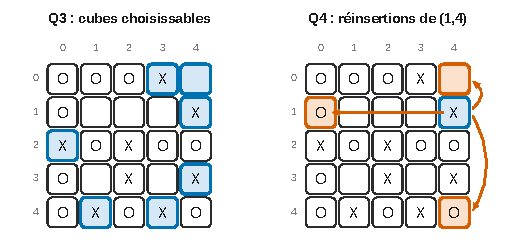
\includegraphics{figures/q3-q4-plateau-figure2.pdf}
\caption*{Figure 1 --- Plateau de la figure 2 : les 7 cubes choisissables par le
joueur 1 (Q3) et les 3 réinsertions du cube (1,4) (Q4)}
\end{figure}

\hypertarget{q5}{%
\subsection{Q5}\label{q5}}

\begin{lstlisting}[language=Python]
def case_bord(i, j):
    return i == 0 or i == 4 or j == 0 or j == 4
\end{lstlisting}

\hypertarget{q6}{%
\subsection{Q6}\label{q6}}

\begin{lstlisting}[language=Python]
def case_choix_valide(jeu, i, j, joueur):
    return case_bord(i, j) and (jeu[i][j] == 0 or jeu[i][j] == joueur)
\end{lstlisting}

\hypertarget{q7}{%
\subsection{Q7}\label{q7}}

D'après le lemme, la nouvelle case est valide dans deux cas :

\begin{itemize}
\tightlist
\item
  elle est sur la même ligne, à une extrémité, et distincte de la case de départ ;
\item
  elle est sur la même colonne, à une extrémité, et distincte de la case de départ.
\end{itemize}

La fonction renvoie directement la disjonction de ces deux conditions.

\begin{lstlisting}[language=Python]
def case_deplacement_valide(i_d, j_d, i_n, j_n):
    meme_ligne = i_n == i_d and (j_n == 0 or j_n == 4) and j_n != j_d
    meme_colonne = j_n == j_d and (i_n == 0 or i_n == 4) and i_n != i_d
    return meme_ligne or meme_colonne
\end{lstlisting}

\hypertarget{q8}{%
\subsection{Q8}\label{q8}}

\emph{Reconstruction du code du cahier de réponses} (structure en quatre cas, boucles \texttt{while}). Les lignes du mouvement 2 sont déjà complétées, ce qui est l'objet de Q9.

\begin{lstlisting}[language=Python]
def deplacement_case(jeu, i_d, j_d, i_n, j_n, joueur):
    if j_n == j_d and i_n == 0:        # mouvement 1
        i = i_d
        while i > 0:
            jeu[i][j_d] = jeu[i - 1][j_d]
            i = i - 1
    elif j_n == j_d and i_n == 4:      # mouvement 2
        i = i_d
        while i < 4:
            jeu[i][j_d] = jeu[i + 1][j_d]
            i = i + 1
    elif j_n == 4:                     # mouvement 3 (i_n == i_d)
        j = j_d
        while j < 4:
            jeu[i_d][j] = jeu[i_d][j + 1]
            j = j + 1
    else:                              # mouvement 4 (i_n == i_d, j_n == 0)
        j = j_d
        while j > 0:
            jeu[i_d][j] = jeu[i_d][j - 1]
            j = j - 1
    jeu[i_n][j_n] = joueur
\end{lstlisting}

\textbf{Mouvement global des pièces.} Dans chaque cas, les cubes situés entre la case d'insertion et la case libérée glissent d'une case vers la case libérée, puis la case d'insertion reçoit la marque du joueur.

\begin{itemize}
\tightlist
\item
  \textbf{Mouvement 1} (insertion en haut de la colonne \(j_d\)) : les cubes des lignes \(0\) à \(i_d-1\) \textbf{descendent} d'une case.
\item
  \textbf{Mouvement 2} (insertion en bas de la colonne) : les cubes des lignes \(i_d+1\) à \(4\) \textbf{montent} d'une case.
\item
  \textbf{Mouvement 3} (insertion à droite de la ligne \(i_d\)) : les cubes des colonnes \(j_d+1\) à \(4\) \textbf{glissent vers la gauche}.
\item
  \textbf{Mouvement 4} (insertion à gauche de la ligne) : les cubes des colonnes \(0\) à \(j_d-1\) \textbf{glissent vers la droite}.
\end{itemize}

\begin{figure}[H]
\centering
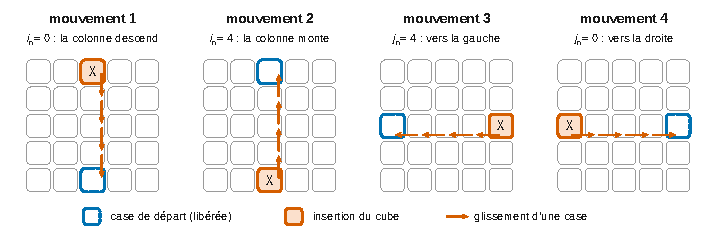
\includegraphics{figures/q8-quatre-mouvements.pdf}
\caption*{Figure 2 --- Les quatre mouvements de deplacement\_case : les cubes
glissent d'une case vers la case libérée}
\end{figure}

\textbf{Terminaison (mouvement 1).} Variant : \(\boxed{V=i}\).

\begin{itemize}
\tightlist
\item
  \(V\) est entier : il vaut \(i_d\in\{0,\dots,4\}\) au départ et n'est modifié que par \texttt{i\ =\ i\ -\ 1}.
\item
  \(V\) est positif : la boucle ne s'exécute que si \(i>0\), donc \(V\ge1\) avant chaque itération.
\item
  \(V\) décroît strictement : chaque itération le diminue de 1.
\end{itemize}

Une suite strictement décroissante d'entiers naturels est finie. La boucle s'arrête donc après \(i_d\le4\) itérations, quand \(i=0\), et la procédure se termine (une seule affectation suit la boucle). L'accès \texttt{jeu{[}i\ -\ 1{]}{[}j\_d{]}} est licite car \(i\ge1\) dans la boucle.

\hypertarget{q9}{%
\subsection{Q9}\label{q9}}

Le mouvement 2 est le symétrique du mouvement 1 : on recopie de bas en haut avec un indice croissant.

\begin{lstlisting}[language=Python]
        i = i_d
        while i < 4:
            jeu[i][j_d] = jeu[i + 1][j_d]
            i = i + 1
\end{lstlisting}

Le variant est \(4-i\), et la boucle fait \(4-i_d\) itérations.

\hypertarget{q10}{%
\subsection{Q10}\label{q10}}

On parcourt la ligne une seule fois en tenant à jour \texttt{c}, le nombre de pions consécutifs du joueur qui se terminent à la case courante.

\begin{lstlisting}[language=Python]
def alig(jeu, joueur, i, n):
    c = 0
    for j in range(5):
        if jeu[i][j] == joueur:
            c = c + 1
            if c == n:
                return True
        else:
            c = 0
    return False
\end{lstlisting}

\textbf{Invariant.} Après le traitement de la colonne \(j\), \texttt{c} est la longueur du bloc maximal de pions du joueur qui se termine en \((i,j)\). Comme \texttt{c} augmente d'une unité à la fois, il atteint \(n\) si et seulement si la ligne contient \(n\) pions consécutifs du joueur. Chaque case est lue une seule fois, d'où au plus 5 accès.

\hypertarget{q11}{%
\subsection{Q11}\label{q11}}

Un alignement gagnant occupe une ligne, une colonne ou une diagonale entière (\(n=5\)).

\begin{lstlisting}[language=Python]
def gagnant(jeu, joueur):
    for k in range(5):
        if alig(jeu, joueur, k, 5) or acol(jeu, joueur, k, 5):
            return True
    return adiag1(jeu, joueur, 5) or adiag2(jeu, joueur, 5)
\end{lstlisting}

\hypertarget{jeu-contre-un-ordinateur}{%
\section{3 Jeu contre un ordinateur}\label{jeu-contre-un-ordinateur}}

\hypertarget{q12}{%
\subsection{Q12}\label{q12}}

\textbf{Situation initiale.} Tous les cubes sont neutres, donc les 16 cases de bord sont disponibles : 4 coins à 2 destinations et 12 autres cases à 3 destinations.
\equationajustee{\boxed{4\times2+12\times3=44\ \text{mouvements.}}}

\textbf{Situation minimale : 4 mouvements.} Exemple pour le joueur 1 : le joueur 2 occupe tout le bord sauf deux coins opposés, \((0,0)\) et \((4,4)\), qui sont neutres.

\begin{longtable}[]{@{}llllll@{}}
\toprule\noalign{}
& 0 & 1 & 2 & 3 & 4 \\
\midrule\noalign{}
\endhead
\bottomrule\noalign{}
\endlastfoot
\textbf{0} & · & O & O & O & O \\
\textbf{1} & O & X & X & · & O \\
\textbf{2} & O & X & · & · & O \\
\textbf{3} & O & · & · & X & O \\
\textbf{4} & O & O & O & O & · \\
\end{longtable}

Aucun joueur n'a d'alignement de 5. Le joueur 1 n'a que deux coins disponibles, soit \(2\times2=\boxed{4}\) mouvements : \((0,0)\to(0,4)\), \((0,0)\to(4,0)\), \((4,4)\to(0,4)\), \((4,4)\to(4,0)\).

Pourquoi on ne peut pas faire moins : avec au plus une case de bord disponible, l'adversaire possède au moins 15 des 16 cases de bord, donc toute la ligne 0 ou toute la ligne 4. Il a alors déjà gagné.

\hypertarget{q13}{%
\subsection{Q13}\label{q13}}

\textbf{Méthode (à appliquer à l'arbre du cahier).} On remonte les valeurs des feuilles vers la racine, niveau par niveau. Chaque nœud MIN (rond) prend le \textbf{minimum} de ses fils et chaque nœud MAX (carré) le \textbf{maximum}. La racine est MAX, puis les niveaux alternent MIN, MAX, MIN jusqu'aux feuilles. Le coup choisi est celui qui mène au fils de valeur maximale.

\textbf{Exemple illustratif} (arbre binaire de même forme, valeurs fictives) :

\begin{figure}[H]
\centering
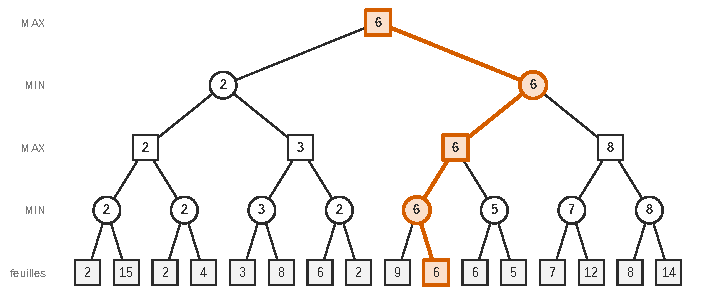
\includegraphics{figures/q13-arbre-minimax.pdf}
\caption*{Figure 3 --- Remontée minimax sur l'arbre illustratif : minimum aux
ronds (MIN), maximum aux carrés (MAX), racine 6}
\end{figure}

Sur cet exemple, on remonte \(\min\) puis \(\max\) niveau par niveau jusqu'à la racine, qui vaut \(\max(2,6)=6\) : MAX choisit la branche droite.

\hypertarget{q14}{%
\subsection{Q14}\label{q14}}

On majore le nombre de mouvements à chaque tour depuis la position initiale.

\begin{itemize}
\tightlist
\item
  \textbf{Tour 1} (joueur 1) : 44 mouvements (Q12).
\item
  \textbf{Tour 2} (joueur 2) : il y a un seul X, sur une case de bord (la case d'insertion). Le joueur 2 peut prendre les 15 autres cases de bord, soit \(44-2=42\) mouvements si le X est sur un coin et \(44-3=41\) sinon. Au plus 42.
\item
  \textbf{Tour 3} (joueur 1) : seul le O, sur le bord, lui est interdit. Au plus 42 mouvements.
\end{itemize}

\equationajustee{\boxed{44\times42\times42=77\,616\approx 8\cdot10^4\ \text{suites de 3 coups au plus.}}}

Le maximum 42 est atteint aux tours 2 et 3 quand le coup précédent a été joué dans un coin. Une énumération exhaustive donne exactement \(76\,596\) suites.

\textbf{Discussion.} Pour une profondeur de 3, explorer environ \(8\cdot10^4\) feuilles (une copie du plateau et une évaluation par nœud) est faisable. Mais le nombre de feuilles croît comme \(b^p\) avec \(b\approx 40\) :

\begin{itemize}
\tightlist
\item
  environ \(4\cdot10^6\) à la profondeur 4 ;
\item
  environ \(7\cdot10^9\) à la profondeur 6.
\end{itemize}

Une partie dure plusieurs dizaines de tours et peut ne jamais finir, puisqu'aucun cube n'est retiré du jeu. \textbf{Le minimax sur l'arbre complet est donc impossible.} On ne peut l'utiliser qu'à faible profondeur, avec une heuristique d'évaluation des feuilles, et on gagne à élaguer l'arbre (alpha-bêta).

\hypertarget{q15}{%
\subsection{Q15}\label{q15}}

\emph{Hypothèse sur le code du cahier.} \texttt{deplacements\_possibles} balaie les cases de départ par lignes puis colonnes croissantes. Pour chaque départ valide, il balaie de même les cases d'arrivée :

\begin{lstlisting}[language=Python]
def deplacements_possibles(jeu, joueur):
    depl = []
    for i in range(5):
        for j in range(5):
            if case_choix_valide(jeu, i, j, joueur):
                for i_n in range(5):
                    for j_n in range(5):
                        if case_deplacement_valide(i, j, i_n, j_n):
                            depl.append([i, j, i_n, j_n])
    return depl
\end{lstlisting}

Sur la figure 3, toutes les cases de bord portent un O, sauf trois X : \((0,3)\), \((2,0)\) et \((4,4)\). Les deux cases neutres, \((1,1)\) et \((1,3)\), sont intérieures. Il y a donc \(3+3+2=8\) mouvements, et la fonction renvoie :
\equationajustee{\boxed{\begin{aligned}\lbrack&[0,3,0,0],\ [0,3,0,4],\ [0,3,4,3],\\ &[2,0,0,0],\ [2,0,2,4],\ [2,0,4,0],\\ &[4,4,0,4],\ [4,4,4,0]]\end{aligned}}}

L'ensemble de ces 8 mouvements ne dépend pas du code. Seul leur ordre dépend du parcours.

\hypertarget{q16}{%
\subsection{Q16}\label{q16}}

Les fonctions de Q10 sont booléennes : on compte les lignes, colonnes et diagonales qui contiennent au moins 4 pions consécutifs du joueur.

\begin{lstlisting}[language=Python]
def alignement_4(jeu, joueur):
    c = 0
    for k in range(5):
        if alig(jeu, joueur, k, 4):
            c = c + 1
        if acol(jeu, joueur, k, 4):
            c = c + 1
    if adiag1(jeu, joueur, 4):
        c = c + 1
    if adiag2(jeu, joueur, 4):
        c = c + 1
    return c
\end{lstlisting}

Le résultat est compris entre 0 et 12.

\hypertarget{q17}{%
\subsection{Q17}\label{q17}}

Le score est orienté vers le joueur 1 (positif s'il gagne, négatif si c'est le joueur 2). Si les deux joueurs sont alignés en même temps, l'énoncé donne la victoire au joueur dont ce n'était pas le tour. Le dernier coup a été joué par l'adversaire de \texttt{joueur} : on lit donc \texttt{joueur} comme le joueur dont c'est le tour, ce qui correspond à l'appel fait dans \texttt{alphabeta}.

\begin{lstlisting}[language=Python]
def evaluation(jeu, joueur, profondeur):
    g1 = gagnant(jeu, 1)
    g2 = gagnant(jeu, 2)
    if g1 and g2:                  # double alignement : gagne le joueur dont c'est le tour
        if joueur == 1:
            return 100 + profondeur
        return -100 - profondeur
    if g1:
        return 100 + profondeur
    if g2:
        return -100 - profondeur
    val = 5 * alignement_4(jeu, joueur) + profondeur
    if jeu[2][2] == joueur:
        val = val + 20
    for i in range(5):
        for j in range(5):
            if jeu[i][j] == joueur:
                val = val + 1
            elif jeu[i][j] != 0:
                val = val - 1
    if joueur == 1:
        return val
    return -val
\end{lstlisting}

Contrôle sur la figure 3, avec une profondeur de 3. Personne n'a gagné.

\begin{itemize}
\tightlist
\item
  \textbf{Joueur 1} : un alignement de 4 (la ligne 2), le centre, 10 X contre 13 O. On obtient \(5+20-3+3=25\), et la fonction renvoie \(25\).
\item
  \textbf{Joueur 2} : deux alignements de 4 (la ligne 4 et la colonne 4), pas le centre. On obtient \(10+3+3=16\), et la fonction renvoie \(-16\).
\end{itemize}

\hypertarget{q18}{%
\subsection{Q18}\label{q18}}

\textbf{Méthode (à appliquer à l'arbre du cahier).} On parcourt l'arbre en profondeur, de gauche à droite, en transmettant l'intervalle \([\alpha,\beta]\) aux fils :

\begin{itemize}
\tightlist
\item
  \(\alpha\) est la meilleure valeur déjà garantie à MAX ;
\item
  \(\beta\) est la meilleure valeur déjà garantie à MIN.
\end{itemize}

Dans un nœud MAX, dès que \(v\ge\beta\), on coupe les fils restants (\textbf{coupure \(\beta\)}). Dans un nœud MIN, dès que \(v\le\alpha\), on coupe (\textbf{coupure \(\alpha\)}). Un nœud coupé ne porte qu'une borne : \(\le v\) pour un nœud MIN, \(\ge v\) pour un nœud MAX.

\textbf{Exemple illustratif} (arbre de Q13). Les branches coupées, qui ne sont pas calculées, sont en pointillé gris.

\begin{figure}[H]
\centering
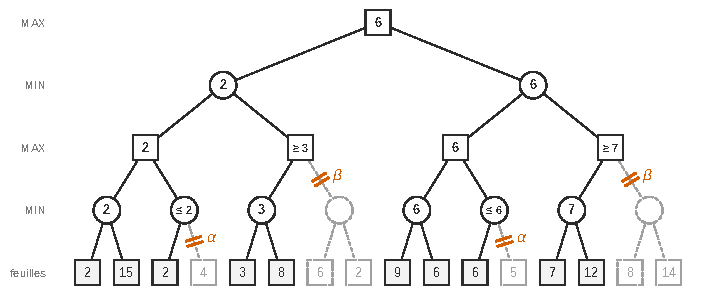
\includegraphics{figures/q18-arbre-alphabeta.pdf}
\caption*{Figure 4 --- Élagage alpha-bêta sur le même arbre, exploré de gauche à
droite : 4 coupures, 10 feuilles évaluées sur 16}
\end{figure}

Les quatre coupures, dans l'ordre de l'exploration :

\begin{itemize}
\tightlist
\item
  sous le deuxième MIN de gauche, la feuille 2 donne \(v=2\le\alpha=2\) : coupure \(\alpha\), la feuille 4 n'est pas lue ;
\item
  le MAX suivant atteint \(3\ge\beta=2\) : coupure \(\beta\), son second fils n'est pas calculé ;
\item
  dans la moitié droite, la feuille 6 donne \(v=6\le\alpha=6\) : coupure \(\alpha\) (feuille 5) ;
\item
  le dernier MAX atteint \(7\ge\beta=6\) : coupure \(\beta\) (feuilles 8 et 14).
\end{itemize}

On trouve la même valeur 6 à la racine, avec 4 coupures et 10 feuilles évaluées sur 16.

\hypertarget{q19}{%
\subsection{Q19}\label{q19}}

\begin{lstlisting}[language=Python]
    if profondeur == 0 or gagnant(jeu, 1) or gagnant(jeu, 2):     # ligne 3
        eval = evaluation(jeu, joueur, profondeur)                 # ligne 4
        return eval, None

            deplacement_case(jeu_c, depl[0], depl[1], depl[2], depl[3], joueur)   # ligne 12
            v = max(v, alphabeta(jeu_c, 2, alpha, beta, profondeur)[0])         # ligne 13
\end{lstlisting}

\begin{itemize}
\tightlist
\item
  \textbf{Ligne 3.} Un nœud est une feuille quand la partie est finie, c'est-à-dire quand un des deux joueurs a gagné. Il y a toujours au moins 4 coups possibles dans une partie non finie (Q12). La profondeur est atteinte quand elle vaut 0.
\item
  \textbf{Ligne 12.} Le coup est joué sur la copie \texttt{jeu\_c}, jamais sur \texttt{jeu}. L'ordre des arguments suit la reconstruction de \texttt{deplacement\_case} de Q8.
\item
  \textbf{Ligne 13.} L'appel récursif porte sur \texttt{jeu\_c}, avec l'adversaire (joueur 2, puisque ce bloc est celui du joueur 1) et la profondeur \textbf{déjà décrémentée} à la ligne 6.
\end{itemize}

\hypertarget{gestion-dune-base-de-donnuxe9es}{%
\section{4 Gestion d'une base de données}\label{gestion-dune-base-de-donnuxe9es}}

\hypertarget{q20}{%
\subsection{Q20}\label{q20}}

\begin{lstlisting}[language=SQL]
SELECT COUNT(*) AS nb_parties, AVG(P.nbtours) AS moyenne_tours
FROM Partie AS P
JOIN Joueur AS J ON P.id_joueur1 = J.id
WHERE J.prenom = 'John' AND J.nom = 'Doe';
\end{lstlisting}

La jointure se fait sur \texttt{id\_joueur1} seulement, ce qui traduit « quand il a commencé la partie ».

\hypertarget{q21}{%
\subsection{Q21}\label{q21}}

\begin{lstlisting}[language=SQL]
SELECT P.nbtours, J1.nom, J1.prenom, J2.nom, J2.prenom
FROM Partie AS P
JOIN Joueur AS J1 ON P.id_joueur1 = J1.id
JOIN Joueur AS J2 ON P.id_joueur2 = J2.id
WHERE P.nbtours = (SELECT MIN(nbtours) FROM Partie);
\end{lstlisting}

La table \texttt{Joueur} est jointe deux fois, sous deux alias, une fois par joueur. Comme la partie minimale est unique, la requête renvoie une seule ligne.

\end{document}
